%%
%%  Department of Electrical, Electronic and Computer Engineering.
%%  EPR400/2 Project Proposal - Section 2.
%%  Copyright (C) 2011-2017 University of Pretoria.
%%

\section{Approach}
In order to fully constrain the system, one actuator is required for every degree of freedom in the system. The robot uses 5 identical legs spaced 72 degrees apart around a circular chassis in order to make the system holonomic. If every leg has N degrees of freedom, the robot will require $5 \times N$ actuators for it to be fully constrained.\\

The robot can be designed with either two or three degrees of freedom per leg. Figure \ref{fig:2DOF} below shows an illustration of a leg with two degrees of freedom. The first hinge can move in the horizontal plane to pivot both segments A and B sideways. The second hinge pivots segment B up and down. The dashed line shows the pivot axes.

\FloatBarrier
\begin{figure}[H]
    \centering
        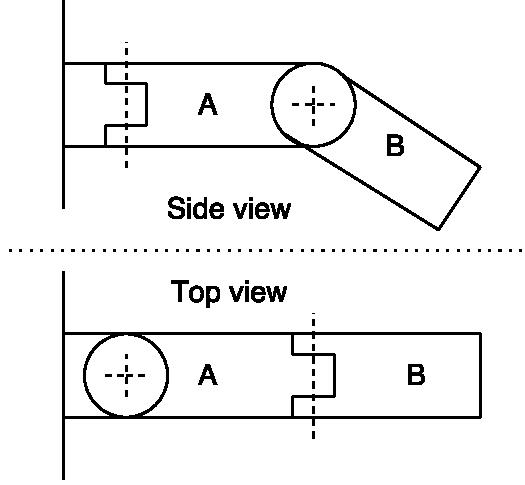
\includegraphics[scale=0.8]{pics/EPR400-2DOF.pdf}
    \caption{Diagram showing a robot leg with two degrees of freedom}
    \label{fig:2DOF}
\end{figure}
\FloatBarrier

Figure \ref{fig:3DOF} below shows an illustration of a robot leg with three degrees of freedom. The first two hinges work the same as in the case of Figure \ref{fig:2DOF} above. The difference is the additional hinge at the end of segment B and the Additional segment C attached to it. The third hinge between segments B and C functions exactly the same as the hinge between segments A and B.

\FloatBarrier
\begin{figure}[H]
    \centering
        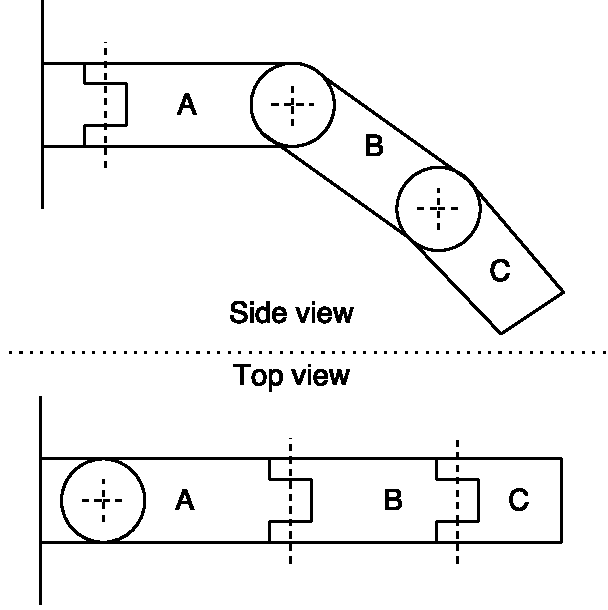
\includegraphics[scale=0.8]{pics/EPR400-3DOF.pdf}
    \caption{Diagram showing a robot leg with three degrees of freedom}
    \label{fig:3DOF}
\end{figure}
\FloatBarrier

If a point with coordinates (x;y;z) is desired, the leg with two degrees of freedom in Figure \ref{fig:2DOF} above will be able to move to a point that satisfies two of the three coordinates. The third is a function of the other two and can therefore not be satisfied without violating one of the other two conditions. The leg in Figure \ref{fig:3DOF} will be able to satisfy all three of these parameters for every set of coordinates within reach of the leg. This leg can move in the X, Y or Z axis without violating the other two parameters.\\

The robot developed in this project should be able to walk on slanted surfaces and rough terrain that includes small obstacles. Control of the Z height of individual legs is therefore important and as a result, the legs should have 3 degrees of freedom each. The robot will therefore require 15 independent actuators to be fully constrained.\\

In section \ref{section:Lit} above, the importance of having feedback on whether a specific leg is touching the surface was discussed. The team in \cite{Ollervides:Navigation} made use of resistive force sensors to determine the exact weight lifting contributed by each leg and therefore the weight distribution of the whole robot. This amount of information is not required in this project. The sole purpose of these sensors in this case is simply to confirm that the leg is touching the surface in order to prevent the robot from falling over. Due to the cost of these resistive force sensors, these will be substituted with simple tactile switches at the bottom of each foot to provide binary information on the feet touching the surface. This will provide all the information necessary to prevent falling over.\\

The importance of having feedback on the current tilt of the robot chassis was also discussed. There are mainly two methods of measuring this digitally. The first method is to use an accelerometer. The earth's gravitational pull will register on the sensor and the tilt of the sensor can be calculated from this. The benefit of using this method is that data on acceleration can be obtained as well. The second method is using a digital inclinometer. This measures the same as the accelerometer but does the conversion calculations on-chip and provides the user with information on tilt in two axes. Since the inclinometer is less expensive and provides the necessary information directly, this will be used in the project.

\newpage

%% End of File.